\documentclass[11pt]{article}

\usepackage[margin=1in]{geometry}
\usepackage{amsmath,amssymb,amsfonts}
\usepackage{times}
\usepackage{graphicx}
\usepackage{booktabs}
\usepackage{longtable}
\usepackage{tikz}
\usetikzlibrary{arrows.meta,positioning,fit,backgrounds,calc}
\usepackage{algorithm}
\usepackage{algpseudocode}
\usepackage{hyperref}
\hypersetup{colorlinks=true,linkcolor=blue,citecolor=blue,urlcolor=blue}
\usepackage[labelfont=bf]{caption}

% --- Supplementary numbering conventions ---
\renewcommand{\theequation}{S\arabic{equation}}
\renewcommand{\thefigure}{S\arabic{figure}}
\renewcommand{\thetable}{S\arabic{table}}
\renewcommand{\thesection}{S\arabic{section}}
\renewcommand{\thealgorithm}{S\arabic{algorithm}}

\newcommand{\chim}{\chi_{m}}

\title{Supplementary Material for:\\
\large ``Worldline Susceptibility as a Surrogate for Spectral Gaps\\ in Quantum Annealing Schedule Design''\\[8pt]
\normalsize The \texttt{qanneal} Library: Theoretical Foundations, Algorithms, and Software}

\author{
Suraj Singh,$^{1,2,3,*}$ Lakshya Nagpal,$^{1,2,3,*}$ Vikas Chauhan,$^{4,2}$ and S.\,R.\ Hassan$^{1,2,5}$\\[4pt]
\small $^{1}$The Institute of Mathematical Sciences (IMSc), C.I.T Campus, Taramani, Chennai 600113, India\\
\small $^{2}$QCAR Group, The Institute of Mathematical Sciences (IMSc), Chennai 600113, India\\
\small $^{3}$Pecslab Research\\
\small $^{4}$Department of Physics, Ramjas College, University of Delhi, Delhi 110007, India\\
\small $^{5}$Homi Bhabha National Institute, Anushakti Nagar, Mumbai, Maharashtra 400094\\[4pt]
\small $^{*}$These authors contributed equally to this work.
}
\date{}

\begin{document}
\maketitle

\begin{abstract}
\noindent
Part of the numerical pipeline behind the main text --- the classical Monte Carlo measurement of
the worldline magnetization susceptibility $\chim$ and the deterministic construction that turns it
into an annealing schedule (main-text Eqs.~7--15) --- was carried out with a worldline-QMC
implementation developed by the authors. This supplement documents that implementation in full,
alongside the statistical-mechanical foundations it rests on. The \emph{other} part of the main
text's pipeline --- exact diagonalization of the spectral gap $\Delta(s)$, the exact Roland--Cerf
schedule built from it, and the unitary/Lindblad time evolution used to compute ground-state
success probabilities --- was produced with separate analysis code that is not part of the software
described here; Sec.~\ref{sec:rc-numerics} states its numerical protocol for completeness but is not
a description of this library. Since the initial submission, the worldline-susceptibility method has
also been generalized into \texttt{qanneal}, an open-source Ising/QUBO annealing library, as a
standalone, production-quality solver (\texttt{method="sqa\_chi"}) applicable to arbitrary dense or
sparse problems, not only the Sherrington--Kirkpatrick ensemble studied here; Sec.~\ref{sec:relation}
states precisely how this released version relates to the analysis that produced the main text's
figures. This supplement is organized the way the library is organized: from the statistical
mechanics every engine rests on, through the five annealing engines it provides, to the
susceptibility-paced adaptive schedule that generalizes the method of the main text. A concordance
table (Sec.~\ref{sec:concordance}) summarizes, item by item, which
main-text results this software did and did not produce, and a condensed API reference and symbol
glossary (Secs.~\ref{sec:api}--\ref{sec:glossary}) close the supplement. \texttt{qanneal} is released
under the Apache License 2.0.
\end{abstract}

\tableofcontents

\section{The Library as This Work's Instrument}
\label{sec:intro}

The central empirical claim of the main text --- that a computationally inexpensive worldline
observable, measured during a classical Monte Carlo simulation, can substitute for the
exponentially expensive spectral gap in annealing schedule design, and can even outperform the
theoretically optimal Roland--Cerf schedule built from that gap --- rests on two logically
separate numerical pipelines. \emph{Only the first is documented in this supplement.}

\begin{enumerate}
\item \textbf{Measuring $\chim$ and constructing the surrogate schedule} (main-text Eqs.~7--15):
a worldline-QMC simulation of the transverse-field Ising model, at a fixed inverse temperature,
used purely to measure $\chim(s)$ and turn it into a schedule. This is what the software described
in this supplement does.
\item \textbf{Grading a schedule} once constructed: exact diagonalization of $\Delta(s)$, the
resulting exact Roland--Cerf schedule (main-text Eq.~20), and unitary/Lindblad propagation of the
Schr\"odinger or Lindblad equation to obtain $P_{\mathrm{GS}}$. This pipeline was implemented with
separate code, is \emph{not} part of the software described here, and is only summarized, for
completeness and not as a specification, in Sec.~\ref{sec:rc-numerics}.
\end{enumerate}

\texttt{qanneal} was built to make step~1 auditable: every knob corresponds to a physical quantity
($\beta$ an inverse temperature, $\Gamma$ a transverse field, $M$ a Trotter number, $J_\perp$ a
Trotter bond strength), schedule endpoints are derived from the problem's own coupling scale rather
than hand-tuned, and every adaptive run exposes its full realized trajectory and observable trace.

The library provides five annealing engines (Table~\ref{tab:engines}) built on a common
statistical-mechanical core, and, on top of them, a schedule that paces the anneal according to
a measured susceptibility rather than a fixed pre-designed ramp: the worldline-magnetization
method, exposed as \texttt{method="sqa\_chi"}, which generalizes the worldline-susceptibility
construction of Section~II of the main text into a standalone, production-quality solver.
Sec.~\ref{sec:relation} states precisely how this released implementation relates to the analysis
that produced the main text's own figures.

\begin{table}[h]
\centering
\caption{The five annealing engines provided by \texttt{qanneal}, and their role in this work.}
\label{tab:engines}
\begin{tabular}{lp{4.6cm}p{4.6cm}}
\toprule
Engine & What it simulates & Role in this work \\
\midrule
\texttt{sa} & Classical thermal (Metropolis) annealing & Encoding sanity checks; not reported \\
\texttt{sqa} & Discrete-time Suzuki--Trotter path integral & Statistical-mechanical core reused by \texttt{sqa\_chi} \\
\texttt{sqapt} & \texttt{sqa} $+$ replica exchange on a $(\beta,\Gamma)$ ladder & Infrastructure for larger-$n$ extensions (Sec.~\ref{sec:sqapt}) \\
\texttt{ctpimc} & Continuous-time (Trotter-error-free) path integral & Infrastructure for larger-$n$ extensions (Sec.~\ref{sec:ctpimc}) \\
\texttt{sqa\_chi} & Worldline-QMC with a $\chim$-measured schedule & \textbf{Generalized, released implementation of the main text's surrogate method} (Sec.~\ref{sec:relation}) \\
\bottomrule
\end{tabular}
\end{table}

\section{Mathematical Foundations: Ising and QUBO}
\label{sec:foundations}

Every problem \texttt{qanneal} solves reduces to one of two energy functions. The Ising form,
which the main text uses throughout,
\begin{equation}
E(s) = \sum_{i=1}^n h_i s_i + \sum_{i<j} J_{ij}s_is_j + c, \qquad s_i\in\{-1,+1\},
\label{eq:ising}
\end{equation}
is what \texttt{DenseIsing(h,J,c)} stores for the fully-connected Sherrington--Kirkpatrick
instances studied in the main text: $h=0$ and $J_{ij}$ drawn i.i.d.\ from a fixed distribution,
with every pair $i<j$ coupled, which is exactly why the library's \texttt{DenseIsing} container
(dense $O(n^2)$ storage, appropriate for $n\lesssim3000$) rather than its sparse counterpart was
used. The library also accepts the equivalent Quadratic Unconstrained Binary Optimization (QUBO)
form over bits $x_i\in\{0,1\}$,
\begin{equation}
E(x) = \sum_{i,j} Q_{ij}x_ix_j,
\label{eq:qubo}
\end{equation}
and converts between the two exactly via the affine map $x_i=(1+s_i)/2$, so that any of the
classic NP-hard encodings the library documents --- number partitioning, MaxCut, and
penalty-constrained problems such as maximum-weight independent set --- can be handed to the
same solvers used for the spin-glass instances of the main text without modification.

The reason any of this is hard is frustration: cycles of bonds whose preferences cannot
simultaneously be satisfied, of which the elementary example is a triangle of antiferromagnetic
couplings. The Sherrington--Kirkpatrick model realizes frustration in its most extreme,
all-to-all form, which is precisely why it was chosen as the benchmark ensemble for the main
text --- it is the setting in which the boundary-gap trap and oscillatory failure modes of
Section~III\,C of the main text are most readily provoked, and in which a schedule's robustness
to those failure modes is most stringently tested.

\section{Statistical Mechanics and the Metropolis Rule}
\label{sec:statmech}

Every engine in the library, quantum or classical, is a Markov-chain Monte Carlo sampler of a
Gibbs--Boltzmann distribution driven slowly toward a zero-temperature or zero-quantum-fluctuation
limit, and it is worth deriving the rule they all share, once, because every acceptance
probability quoted below --- for the classical spin flip, for the Suzuki--Trotter slice flip, for
the parallel-tempering swap, and for the parity-parallel checkerboard sweep that measures
$\chim(s)$ in the main text --- is a special case of it.

A system with energy function $E$ held at inverse temperature $\beta=1/k_BT$ occupies
configuration $s$ with probability $\pi_\beta(s)=e^{-\beta E(s)}/Z(\beta)$. Sampling this
distribution directly at the large $\beta$ needed for optimization is as hard as the optimization
problem itself, so annealing instead walks a Markov chain whose transition kernel satisfies
detailed balance, $\pi(s)P(s\to s') = \pi(s')P(s'\to s)$, and slowly cools $\beta$ (or, in the
quantum engines, slowly raises $J_\perp$) while the chain tracks the shifting equilibrium.
Factoring the transition into a symmetric proposal (pick a spin, or a slice, or a ladder rung, and
propose flipping or exchanging it) and an acceptance probability $A$, detailed balance forces
$A(s\to s')/A(s'\to s) = e^{-\beta\Delta E}$, and the choice that maximizes the acceptance rate
--- and hence mixing speed --- is the Metropolis rule,
\begin{equation}
A(s\to s') = \min\!\big(1,\, e^{-\beta\Delta E}\big).
\label{eq:metropolis}
\end{equation}
Every C++ core in the library executes exactly Eq.~\eqref{eq:metropolis} (or its imaginary-time
generalization, Sec.~\ref{sec:sqa}); a cached local field $f_i=h_i+\sum_j J_{ij}s_j$ makes the
energy change of a single-spin proposal an $O(1)$ evaluation, $\Delta E_i=-2s_if_i$, and this
caching is the single implementation detail most responsible for the library's sweep throughput,
including the throughput of the released \texttt{sqa\_chi} pilot scan described in
Sec.~\ref{sec:sqachi}.

\section{Engine I --- Simulated Annealing (\texttt{sa})}
\label{sec:sa}

The classical baseline runs Metropolis dynamics under a rising-$\beta$ schedule and is not used
for any result reported in the main text. It is documented here because it is the library's
simplest encoding sanity check: for a new problem class, solving small instances ($n\lesssim20$)
by \texttt{sa} and, where feasible, by brute force, is the recommended way to catch an encoding
error before trusting any downstream spectral-gap or susceptibility calculation built on top of
it; whether this specific check was applied to the Sherrington--Kirkpatrick instances of the main
text is not verified in this supplement. Problem-adaptive tuned schedules
(\texttt{auto\_schedule\_sa\_tuned}) remove the need to hand-choose $\beta_{\rm start}$ and
$\beta_{\rm end}$: they probe the problem's own energy scale $\Delta$ (the 75th percentile of
$|\Delta E|$ over random single-spin flips) and invert the acceptance-targeting relation
$\beta(p)=-\ln p/\Delta$ to hit prescribed start/end acceptance rates. This probe-and-invert
pattern reappears, essentially unchanged, in the tuned schedules for every quantum engine below,
including the endpoints of the pilot scan that estimates $\chim(s)$ in Sec.~\ref{sec:sqachi}.

\section{Engine II --- Simulated Quantum Annealing (\texttt{sqa}) and the Suzuki--Trotter Mapping}
\label{sec:sqa}

This is the engine whose statistical mechanics the main text's central observable is built from,
and it is worth re-deriving the mapping in full, because Eqs.~(5)--(6) of the main text are
literally the output of the derivation below.

\subsection{From the transverse-field Ising model to a classical action}
Quantum annealing encodes the optimization problem in the transverse-field Ising Hamiltonian
$\hat H(\Gamma) = \hat H_{\rm cl} - \Gamma\sum_i\hat\sigma_i^x$, where $\hat H_{\rm cl}$ is
diagonal in the computational basis and is exactly Eq.~\eqref{eq:ising}. Real-time simulation of
this Hamiltonian is exponentially expensive, so \texttt{sqa} instead samples its \emph{thermal
equilibrium} at inverse temperature $\beta$ via a mapping onto an equivalent classical system that
Monte Carlo can handle. Trotterizing $e^{-\beta\hat H}=\big(e^{-\frac{\beta}{M}\hat H}\big)^M$ and
splitting each thin slice, $e^{-\frac{\beta}{M}(\hat H_{\rm cl}+\hat H_q)} \approx
e^{-\frac{\beta}{M}\hat H_{\rm cl}}e^{-\frac{\beta}{M}\hat H_q}$, with an error of
$O(\beta^2/M^2)$ per slice that vanishes as the Trotter number $M\to\infty$; inserting a complete
set of classical states between every factor and using the cyclicity of the trace turns the
quantum partition function into a sum over $M$ classical replicas ("slices") of the original spin
configuration. The transverse factor between adjacent slices reduces, site by site, to a $2\times2$
transfer matrix $\langle s|e^{a\hat\sigma^x}|s'\rangle$ with $a=\beta\Gamma/M$, which can be
rewritten as an ordinary classical Ising bond $\Lambda\,e^{J_\perp s s'}$ provided
\begin{equation}
J_\perp(\beta,\Gamma,M) = \frac{1}{2}\ln\coth\!\Big(\frac{\beta\Gamma}{M}\Big)
= \frac12\ln\frac{1}{\tanh(\beta\Gamma/M)},
\label{eq:jperp}
\end{equation}
which is exactly Eq.~(6) of the main text's $J_\perp(\beta,\Gamma)$. Substituting back gives the
effective classical action executed by the C++ core,
\begin{equation}
S[s] = \frac{\beta}{M}\sum_{t=1}^M E_{\rm cl}(s^t) - J_\perp\sum_{t=1}^M\sum_{i=1}^n s_i^t s_i^{t+1},
\label{eq:seff}
\end{equation}
identical to Eq.~(5) of the main text: $M$ replicas of the classical problem, each internally
coupled by the rescaled problem couplings $\frac{\beta}{M}J_{ij}$, and neighbouring replicas tied
site-by-site along imaginary time by the Trotter bond $J_\perp$. Because $J_\perp$ decreases
monotonically as $\Gamma$ increases, an annealing run that lowers $\Gamma$ from a large initial
value corresponds to \emph{raising} $J_\perp$ from near zero (decoupled, freely fluctuating
slices, $\Gamma\to\infty$) to a large value (locked, classical slices, $\Gamma\to0^+$); every
adaptive-schedule interface in the library is parameterized by $J_\perp$ for this reason, and
Fig.~\ref{fig:trotter} sketches the lattice this action describes.

\begin{figure}[h]
\centering
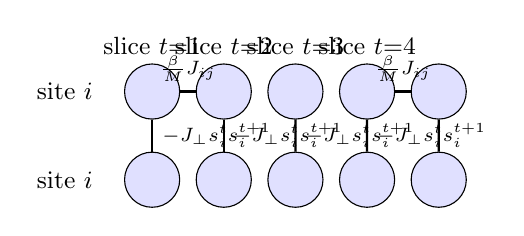
\begin{tikzpicture}[scale=0.7,every node/.style={font=\small}]
  \foreach \c in {0,...,4}{
      \node[draw,circle,fill=blue!12,minimum size=0.7cm] (a\c) at (\c*1.3,0) {};
  }
  \foreach \c in {0,3}{
      \pgfmathtruncatemacro{\cn}{\c+1}
      \draw[thick] (a\c) -- (a\cn) node[midway,above]{\scriptsize $\frac{\beta}{M}J_{ij}$};
  }
  \node[above] at (0,0.5) {slice $t{=}1$};
  \node[above] at (1.3,0.5) {slice $t{=}2$};
  \node[above] at (2.6,0.5) {slice $t{=}3$};
  \node[above] at (3.9,0.5) {slice $t{=}4$};
  \foreach \c in {0,...,4}{
      \node[draw,circle,fill=blue!12,minimum size=0.7cm] (b\c) at (\c*1.3,-1.6) {};
  }
  \foreach \c in {0,1,2,3}{
      \draw[thick] (a\c)--(b\c) node[midway,right]{\scriptsize $-J_\perp s_i^t s_i^{t+1}$};
  }
  \draw[thick] (a4)--(b4);
  \node[left] at (-0.9,0) {site $i$};
  \node[left] at (-0.9,-1.6) {site $i$};
\end{tikzpicture}
\caption{The Suzuki--Trotter lattice underlying Eqs.~\eqref{eq:jperp}--\eqref{eq:seff} (and
Eqs.~(5)--(6) of the main text): replicas of the classical problem coupled within a slice by the
rescaled problem couplings, and coupled to their imaginary-time neighbours by $J_\perp$. The
worldline-magnetization order parameter $m$ of Eq.~(7) of the main text is the mean spin over
this entire two-dimensional lattice.}
\label{fig:trotter}
\end{figure}

\subsection{Monte Carlo moves and why more than one move type is needed}
The \texttt{SQAAnnealer} mixes three move types, all satisfying detailed balance for
Eq.~\eqref{eq:seff}: single-spin (slice) flips, whose action change has a classical part and a
quantum part from the two adjacent time-bonds, $\Delta S=\frac{\beta}{M}\Delta E_{\rm cl} +
2J_\perp s_i^t(s_i^{t-1}+s_i^{t+1})$; whole-worldline flips, which flip one site in every slice
simultaneously so that every imaginary-time bond touching it is a product of two flipped spins
and therefore invariant, leaving $\Delta S_{\rm worldline}=\frac{\beta}{M}\sum_t\Delta
E_{\rm cl}^{(t)}$ with no Trotter penalty at all; and Swendsen--Wang cluster moves along
imaginary time, which grow a contiguous worldline segment with join probability
$p_{\rm join}=1-e^{-2J_\perp}$ and flip it as a unit. Single-spin flips alone become
exponentially inefficient once $J_\perp$ is large (deep in the anneal, exactly where the
susceptibility scan of Sec.~\ref{sec:sqachi} needs to equilibrate quickly), because $\Delta S
\approx4J_\perp$ for a lone slice flip; worldline flips pay no such penalty and are essential
late in the anneal, while cluster moves interpolate between the two extremes and are the
recommended addition (\texttt{cluster\_sweeps=1}, the ``+SW'' variant) whenever a run visibly
stalls. This mix of move types is the reason a $\chim(s)$ measurement equilibrates within the
modest \texttt{scan\_burn}$+$\texttt{scan\_sweeps} budget used for the pilot scan in
Sec.~\ref{sec:sqachi}, rather than requiring the enormous sweep counts a single-spin-only sampler
would need at large $J_\perp$.

\section{Engine III --- Quantum Parallel Tempering (\texttt{sqapt})}
\label{sec:sqapt}

\texttt{sqapt} runs $R$ complete Suzuki--Trotter systems simultaneously on a $(\beta,\Gamma)$
ladder and periodically proposes exchanging full configurations between adjacent rungs, with a
swap acceptance
\begin{equation}
A_{\rm swap} = \min\!\Big(1,\ \exp\!\big[-\big(S_r(x_{r+1})+S_{r+1}(x_r)-S_r(x_r)-S_{r+1}(x_{r+1})\big)\big]\Big)
\label{eq:sqapt-swap}
\end{equation}
derived from detailed balance on the joint product measure over all rungs. Expanding
Eq.~\eqref{eq:sqapt-swap}, the swap criterion splits cleanly into a thermal part (the ordinary
classical parallel-tempering criterion applied to slice-summed energies) and a quantum part
proportional to $J_\perp^{(r)}-J_\perp^{(r+1)}$; when every rung shares a single evolving
$J_\perp$, the quantum part vanishes identically and the swap reduces to the classical criterion
alone. \texttt{sqapt} was not used to
generate any of the main text's reported ground-state probabilities --- those come from direct
propagation of the time-dependent Schr\"odinger equation under exact diagonalization, so as to
compare schedules on identical footing without introducing additional sampling noise --- but it
is the natural engine for the disorder-averaged, larger-$n$ extensions the current publishability
assessment of this project calls for: replica exchange is the standard remedy when read-to-read
variance is large, which is exactly the symptom the main text's Fig.~7 shows growing with $n$ for
the Roland--Cerf schedule.

\section{Engine IV --- Continuous-Time Path-Integral Monte Carlo (\texttt{ctpimc})}
\label{sec:ctpimc}

Taking $M\to\infty$ at fixed $\beta$ in Eq.~\eqref{eq:seff} turns the discrete slice index into a
continuous imaginary time $\tau\in[0,\beta)$ and each spin into a piecewise-constant worldline
with kinks (domain walls in time) occurring as a Poisson process of rate $\Gamma$; the partition
function becomes $Z=\sum_{\rm configs} \Gamma^K \exp[-\int_0^\beta E_{\rm cl}(s(\tau))\,d\tau]$,
with $K$ the total kink count, and the engine's Swendsen--Wang-style cluster updates act directly
on worldline segments with no discretization scale at all. \texttt{qanneal}'s implementation
builds on D-Wave's open-source \texttt{localPIMC} code (Apache-2.0, credited in the repository's
NOTICE file). This engine removes the systematic Trotter error of Sec.~\ref{sec:sqa} entirely and
is the natural choice if a future extension of this work were to ask whether any of the
Roland--Cerf failure modes of Section~III\,C of the main text are sensitive to the residual
$O(\beta^2\Gamma^2/M)$ discretization error of \texttt{sqa} --- a question the present results
already answer in the negative for the parameter ranges studied (the solver-tolerance sweep of
Sec.~\ref{sec:rc-numerics}), but one for which \texttt{ctpimc} provides an independent,
discretization-free cross-check.

\section{The Worldline-Susceptibility Schedule (\texttt{sqa\_chi})}
\label{sec:sqachi}

This section describes the released, generalized software implementation of the method the main
text is about; Sec.~\ref{sec:relation} states exactly how it relates to the analysis that produced
the main text's own figures. \texttt{sqa\_chi} is a standalone solver
class, \texttt{SQAChiAnnealer}, that measures the worldline magnetization
\begin{equation}
m = \frac{1}{nM}\sum_{i=1}^n\sum_{k=1}^M \sigma_i^k, \qquad
\chim = nM\big(\langle m^2\rangle - \langle|m|\rangle^2\big),
\label{eq:chim-def}
\end{equation}
identical to Eqs.~(7)--(8) of the main text, and paces the anneal in the annealing parameter $s$
of Eq.~(16) of the main text rather than in $J_\perp$ directly, via $s=A_0/(A_0+\Gamma)$ with
$A_0$ the driver scale.

\subsection{The pilot scan}
At \texttt{scan\_points} (default 16) values of $s$ spanning the annealing interval, the solver
equilibrates a freshly and independently randomized worldline for \texttt{scan\_burn} (default
10) sweeps and measures $\chim$ over the next \texttt{scan\_sweeps} (default 30) sweeps, using the
parity-parallel checkerboard kernel described below. Each grid point is deliberately \emph{not}
carried forward from the previous one: a carried-over scan would gently anneal itself as it
proceeds, correlating each susceptibility estimate with the point before it and making the
resulting peak location harder to trust as an independent measurement. This is the same protocol
--- pilot scan at a sequence of $s$ values, each from an independently randomized worldline --- as
the one that located $s^*_{\rm SQ}=0.920$ (the $n=10$ instance) and $s^*_{\rm SQ}=0.876$ (the
$n=12$ instance) of the main text's Table~I, against the exact-diagonalization gap minima
$s^*_{\rm ED}=0.883$ and $1.000$ respectively; see Sec.~\ref{sec:relation} for the precise
relationship between this released implementation and the code that produced those specific
numbers.

\subsection{From the scan to a schedule: floor regularization and inverse-CDF placement}
The scan profile is turned into a schedule exactly as Eqs.~(11)--(14) of the main text describe,
with one implementation specialization: the released solver applies a multiplicative floor,
\begin{equation}
w(s)=\max\bigl(\chim(s),\,\text{floor}\bigr),
\qquad
\text{floor}=\max\bigl(f\cdot\max_s\chim(s),\,10^{-12}\bigr),
\label{eq:floor-note}
\end{equation}
with $f=$~\texttt{chi\_floor\_fraction} (default $10^{-6}$), rather than the additive constant
$\chi_0$ of Eq.~(11). The two play the same regularizing role, but the multiplicative floor is
scale-invariant across problem sizes: because $\chim\sim O(nM)$, a fixed additive constant tuned
for the $n=10$ instance of Fig.~1 would be numerically negligible for a larger ensemble member
and disastrously large for a smaller one, whereas a floor defined as a fixed fraction of each
instance's own scan peak automatically rescales with the problem --- a design choice intended to
make the released solver usable, unmodified, across a wide range of system sizes without
per-instance retuning, of the kind spanned by the $n\in\{10,\dots,20\}$ ensemble of Figs.~7--9 of
the main text (whether the original analysis code used this exact regularization for those figures
is not verified here; see Sec.~\ref{sec:relation}).
$\chim(s)$ is linearly interpolated between scan points and clamped outside $[s_{\rm lo},s_{\rm
hi}]$; the cumulative integral $\tau(s)$ is evaluated by trapezoidal quadrature on a 4096-point
grid and inverted to place each remaining step at an equal increment of accumulated weight. If
the pilot scan is flat or non-finite --- the \texttt{sqa\_chi} analogue of the boundary-gap
degeneracy discussed for Roland--Cerf in Section~III\,C\,1 of the main text --- the floor falls
back to $1$, $w(s)$ becomes uniform, and the schedule degrades gracefully to a linear-in-$s$ ramp
rather than failing.

\subsection{The parity-parallel checkerboard kernel}
\label{sec:kernel-note}
Every sweep in \texttt{sqa\_chi}, pilot or production, exploits a structural fact about
Eq.~\eqref{eq:seff}: Trotter slices of the same parity are never directly coupled, since the
imaginary-time bond only ever links a slice to its opposite-parity neighbours. Held one parity
fixed, every $(\text{replica},\text{slice})$ cell of the other parity can therefore be updated by
an independent, ordinary sequential single-spin Metropolis sweep, dispatched to a single OpenMP
parallel loop; two such passes (even, then odd) constitute one full sweep of the lattice
(Algorithm~\ref{alg:checkerboard}, Fig.~\ref{fig:checkerboard}). This is why \texttt{sqa\_chi}
parallelizes usefully even at \texttt{replicas=1}, unlike every other engine in the library, whose
OpenMP parallelism is over replicas alone and is therefore inert for a single-replica run.

A tempting shortcut --- flip an entire slice's spins simultaneously, using the previous sweep's
neighbour-slice values for the in-plane coupling --- is exact detailed balance only when the
\emph{spatial} coupling graph is bipartite. The Sherrington--Kirkpatrick instances of the main
text are fully connected and maximally frustrated, so this shortcut would silently bias the
sampled distribution for exactly the problem class studied here. The released implementation
therefore uses the sequential per-slice update of Algorithm~\ref{alg:checkerboard}, which is exact
for an arbitrary coupling graph while still parallelizing across slices; this is a deliberate
robustness improvement made when generalizing the method for public release
(Sec.~\ref{sec:relation}), not a claim about the exact update rule used in the original analysis
that produced the main text's figures.

\begin{algorithm}[h]
\caption{One sweep of the parity-parallel checkerboard kernel underlying \texttt{sqa\_chi}}
\label{alg:checkerboard}
\begin{algorithmic}[1]
\Require Trotter lattice of $R$ replicas $\times$ $M$ slices $\times$ $n$ spins; cached local fields
\For{\textbf{parity} $\in \{\text{even}, \text{odd}\}$}
    \State \textbf{parallel for} every $(r,t)$ with $t\bmod2=\text{parity}$:
    \Statex \hspace{1.5em} run a full sequential single-spin Metropolis sweep over the $n$ spins of slice $t$, replica $r$,
    \Statex \hspace{1.5em} using the classical-plus-Trotter action change of Sec.~\ref{sec:sqa} and the cached local fields of Sec.~\ref{sec:statmech};
    \Statex \hspace{1.5em} update the cache and the incremental bond sum $B$ on every accepted flip.
\EndFor
\State \Return pooled worldline magnetization $m$ [Eq.~\eqref{eq:chim-def}] across all $(r,t)$
\end{algorithmic}
\end{algorithm}

\begin{figure}[h]
\centering
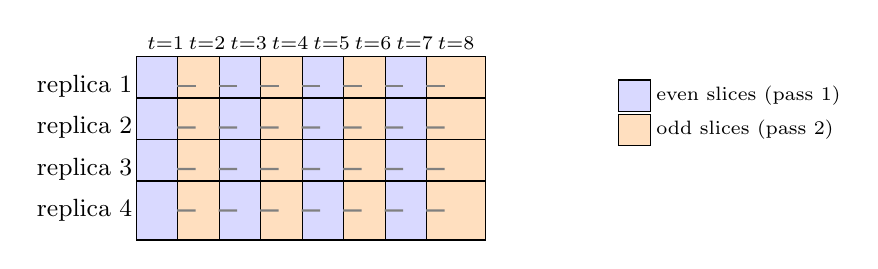
\begin{tikzpicture}[scale=0.62,every node/.style={font=\small}]
  \foreach \r in {0,...,3}{
    \foreach \c in {0,...,7}{
      \pgfmathtruncatemacro{\isEven}{mod(\c,2)}
      \ifnum\isEven=0
        \node[draw,fill=blue!15,minimum size=0.75cm] (n\r-\c) at (\c*0.85,-\r*0.85) {};
      \else
        \node[draw,fill=orange!25,minimum size=0.75cm] (n\r-\c) at (\c*0.85,-\r*0.85) {};
      \fi
    }
  }
  \foreach \r in {0,...,3}{
    \foreach \c in {0,...,6}{
      \pgfmathtruncatemacro{\cnext}{\c+1}
      \draw[thick,gray] (n\r-\c) -- (n\r-\cnext);
    }
  }
  \node[left=0.3cm] at (0,-0*0.85) {replica 1};
  \node[left=0.3cm] at (0,-1*0.85) {replica 2};
  \node[left=0.3cm] at (0,-2*0.85) {replica 3};
  \node[left=0.3cm] at (0,-3*0.85) {replica 4};
  \node[above] at (0*0.85,0.55) {\scriptsize $t{=}1$};
  \node[above] at (1*0.85,0.55) {\scriptsize $t{=}2$};
  \node[above] at (2*0.85,0.55) {\scriptsize $t{=}3$};
  \node[above] at (3*0.85,0.55) {\scriptsize $t{=}4$};
  \node[above] at (4*0.85,0.55) {\scriptsize $t{=}5$};
  \node[above] at (5*0.85,0.55) {\scriptsize $t{=}6$};
  \node[above] at (6*0.85,0.55) {\scriptsize $t{=}7$};
  \node[above] at (7*0.85,0.55) {\scriptsize $t{=}8$};
  \node[draw,fill=blue!15,minimum size=0.4cm] (legA) at (9.6,-0.2) {};
  \node[right] at (9.85,-0.2) {\scriptsize even slices (pass 1)};
  \node[draw,fill=orange!25,minimum size=0.4cm] (legB) at (9.6,-0.9) {};
  \node[right] at (9.85,-0.9) {\scriptsize odd slices (pass 2)};
\end{tikzpicture}
\caption{The checkerboard decomposition of Algorithm~\ref{alg:checkerboard}. Grey lines are the
imaginary-time Trotter bonds of Fig.~\ref{fig:trotter}; because they always connect
opposite-parity slices, one parity can be updated in a single independent parallel pass while the
other is held fixed.}
\label{fig:checkerboard}
\end{figure}

\subsection{Two-phase protocol and production anneal}
The first $\lceil\text{\texttt{beta\_ramp\_fraction}}\cdot T\rceil$
steps (default fraction $0.3$) ramp $\beta$ from a hot starting value to the cold target at fixed
$\gamma=\gamma_{\rm start}$; the remaining steps hold $\beta$ fixed and follow the calibrated
$\gamma(s_k)$ trajectory, and the solver returns its own best-energy classical configuration found
along the way. Both the pilot scan and this production anneal run on independent, freshly
initialized worldlines, so a \texttt{sqa\_chi} run's own classical result is not contaminated by
state carried over from the diagnostic scan that located the critical region in the first place.
Note that this classical SQA production anneal is a separate, self-contained solve --- it is
\emph{not} the source of the ground-state probabilities $P_{\rm GS}$ reported in Figs.~3--10 of
the main text, which instead come from the exact unitary evolution described in
Sec.~\ref{sec:rc-numerics}, using the schedule $s(t)$ that the pilot scan and the cumulative-weight
construction of Eqs.~(11)--(14) of the main text determine.

\section{Relationship Between This Release and the Main Text's Original Analysis}
\label{sec:relation}

The worldline-susceptibility measurement and schedule-construction algorithm of
Sec.~\ref{sec:sqachi} (main-text Eqs.~7--15) is the same procedure, and uses the same governing
equations, as the one that produced the main text's $\chim(s)$ measurements, critical-point
estimates, and resulting schedules (Fig.~1, Fig.~2, Table~I, and the schedules underlying
Figs.~3--10). It is \emph{not}, however, literally the same code. The analysis reported in the
main text was carried out with an earlier, problem-specific research script written to validate
the method on the Sherrington--Kirkpatrick ensemble. The \texttt{SQAChiAnnealer} class and
\texttt{method="sqa\_chi"} solver described in this supplement are a subsequent, generalized
C++/Python reimplementation of that same method, prepared for the public release of
\texttt{qanneal} so that the method is usable on arbitrary dense or sparse Ising and QUBO problems
rather than only the SK instances studied here. Concretely:

\begin{itemize}
\item The governing equations (worldline magnetization and susceptibility, Eq.~\eqref{eq:chim-def};
the annealing-parameter mapping $s=A_0/(A_0+\Gamma)$; the cumulative-weight schedule construction)
are identical between the original analysis and the released solver.
\item The released solver's update kernel (the parity-parallel checkerboard sweep,
Sec.~\ref{sec:kernel-note} below and Algorithm~\ref{alg:checkerboard}) generalizes the update rule
used in the original analysis to arbitrary, non-bipartite coupling graphs; for the fully-connected
Sherrington--Kirkpatrick instances of the main text the two are expected to sample the same
equilibrium distribution but are not bit-for-bit identical programs.
\item The released solver's regularization (the multiplicative floor of Eq.~\eqref{eq:floor-note}
below) and its independently-re-randomized pilot scan are engineering choices made for robustness
across arbitrary problem sizes; whether the original analysis used precisely these choices or
close variants of them was not re-verified for this supplement.
\item Table~\ref{tab:repro} therefore reports the released solver's \emph{default} configuration
for this method, not a verified record of the exact parameters used to produce any specific
main-text figure.
\end{itemize}

We report the released implementation in full, rather than only the original research script,
because it is the version intended for reuse and independent verification of the method itself;
readers wishing to exactly reproduce a specific main-text figure bit-for-bit should treat this
supplement as a specification of the \emph{method}, not as the literal analysis code.

\section{Numerical Protocol for the Reference Roland--Cerf Schedule}
\label{sec:rc-numerics}

For completeness, we document here the numerical protocol used to generate the exact
Roland--Cerf reference schedule and ground-state probabilities against which the library's
surrogate is judged, since these were produced outside \texttt{qanneal} proper (by direct exact
diagonalization and time-dependent Schr\"odinger-equation propagation) and their reliability is
essential context for interpreting every figure in Section~III of the main text. Spectral data
($\Delta(s)$ and the transition matrix element of Eq.~(4)) were obtained for each disorder
realization by full exact diagonalization of $H(s)$ on a dense grid of $s$ (400--800 points,
refined adaptively near the minimum gap); ground-state success probabilities were obtained by
adaptive-step Runge--Kutta (embedded Dormand--Prince) integration of the Schr\"odinger equation
under each schedule, with tolerances swept over $10^{-8}$--$10^{-12}$ and the schedule's own
internal discretization varied independently, in order to test the oscillatory Roland--Cerf
failure mode of Section~III\,C\,2 of the main text for solver artifacts; the oscillation period
and amplitude were unchanged to within machine precision across this entire sweep. The Lindblad
robustness check of Section~III\,F integrates $\dot\rho=-i[H(s(t)),\rho]+\sum_k\gamma\,
\mathcal D[\sigma_z^{(k)}]\rho$ for the same representative instance at dephasing rates
$\gamma\in\{0,10^{-3},10^{-2},5\times10^{-2}\}$ with a fixed-step fourth-order Runge--Kutta
propagator of the vectorized Liouvillian.

\section{Parallel and HPC Deployment}
\label{sec:hpc}

This section describes the released library's parallel-execution capability, of the kind suited to
disorder-averaged ensembles such as Figs.~7--9 of the main text (20--100 independent
Sherrington--Kirkpatrick instances per system size, across six system sizes); it is not a record of
the specific hardware or job configuration used for those particular figures (Sec.~\ref{sec:relation}).
\texttt{qanneal} supports three nested levels of parallelism: OpenMP threads within a single
\texttt{sqa\_chi} pilot scan or run (parallel over replicas, and, uniquely for this engine, over
Trotter slices as well, Sec.~\ref{sec:sqachi}); independent worker processes distributing reads and
disorder realizations across the cores of a single node; and SLURM job arrays distributing
realizations across nodes of an HPC cluster (the \texttt{nandadevi} and \texttt{kamet} clusters at
IMSc were used for other benchmarking of this library, not verified here as the specific resource
behind any main-text figure), one array task per disorder seed, mergeable afterward into ensemble
statistics of the form of Eq.~\eqref{eq:sem} below. The job-array route is preferred by the library's
own documentation over a long-running MPI job for the usual reason: a failed task costs one disorder
realization, not the whole ensemble. Reproducibility of a \texttt{sqa\_chi} run only requires
recording the random seed and the solver configuration (cf.\ Table~\ref{tab:repro} for the released
defaults); OpenMP thread count and process count do not affect the result, since each parallel unit
owns a private RNG stream, local-field cache, and cluster buffers.

\section{Concordance: Main-Text Results and the Methods Behind Them}
\label{sec:concordance}

Table~\ref{tab:concordance} maps every quantitative result in Sections~II--III of the main text to
the \emph{method} responsible for it, and states plainly whether that method is one this
supplement documents in software form (worldline-susceptibility measurement and schedule
construction, Secs.~\ref{sec:sqa}--\ref{sec:sqachi}) or one that is outside its scope (exact
diagonalization, unitary/Lindblad evolution, disorder averaging over independently generated
realizations). Per Sec.~\ref{sec:relation}, entries in the third column naming \texttt{sqa\_chi}
or \texttt{SQAChiAnnealer} refer to the method and its released, generalized implementation, not a
verified record of the literal code that ran for the main text.

\begin{table}[h]
\centering
\small
\caption{Concordance between main-text results and the methods that produced them.}
\label{tab:concordance}
\begin{tabular}{p{3.3cm}p{3.6cm}p{6.3cm}}
\toprule
Main-text item & Equation(s) & Method (software scope, if any) \\
\midrule
Fig.~1, Table~I ($s^*_{\rm SQ}$) & Eqs.~(7)--(9) & Worldline-susceptibility pilot scan; released as \texttt{SQAChiAnnealer} (Sec.~\ref{sec:sqachi}) \\
Fig.~2 (schedule shapes) & Eqs.~(11)--(15) & Cumulative-weight inverse-CDF construction; released as \texttt{sqa\_chi} (Sec.~\ref{sec:sqachi}) \\
Figs.~3--10 ($P_{\rm GS}$ vs.\ $T$) & Eqs.~(18)--(19) & Exact diagonalization $+$ TDSE propagation (\emph{not} part of this software); driven by the critical-region estimate of Fig.~1 (Sec.~\ref{sec:rc-numerics}) \\
Fig.~5, Eq.~(20) (RC cumulative allocation) & Eq.~(20) & Exact-diagonalization $\Delta(s)$; outside this software's scope \\
Fig.~6 (RC oscillation) & --- & Solver-tolerance sweep on the TDSE propagator; outside this software's scope (Sec.~\ref{sec:rc-numerics}) \\
Figs.~7--9 (disorder averages) & Eq.~\eqref{eq:sem} & Ensemble statistics over independently generated SK realizations; outside this software's scope \\
Fig.~12 (failure-class fractions) & --- & Classification protocol applied to the Figs.~7--9 ensemble; outside this software's scope \\
Fig.~13 (Lindblad) & Eq.~(21) & Lindblad propagator; outside this software's scope (Sec.~\ref{sec:rc-numerics}) \\
Figs.~14--15 ($\beta,M$ robustness) & --- & Worldline-susceptibility pilot scan swept over $M,\beta$; released as \texttt{SQAChiAnnealer} \\
\bottomrule
\end{tabular}
\end{table}

\begin{equation}
{\rm SEM}(T) = \frac{1}{\sqrt{N_{\rm inst}}}
\sqrt{\frac{1}{N_{\rm inst}-1}\sum_{a=1}^{N_{\rm inst}}\big(P_{\rm GS}^{(a)}(T)-\overline P_{\rm GS}(T)\big)^2}
\label{eq:sem}
\end{equation}

Table~\ref{tab:repro} records the released \texttt{sqa\_chi} solver's \emph{default}
configuration for this method (Sec.~\ref{sec:relation}); parameters not listed were left at their
library defaults (Sec.~\ref{sec:api}).

\begin{table}[h]
\centering
\caption{Default \texttt{sqa\_chi} solver configuration in the current \texttt{qanneal} release (Sec.~\ref{sec:relation}).}
\label{tab:repro}
\begin{tabular}{ll}
\toprule
Parameter & Value \\
\midrule
\texttt{trotter\_slices} ($M$) & 32 \\
\texttt{replicas} & 4 \\
\texttt{optimal\_num\_steps} (step budget $T$) & 150 \\
\texttt{optimal\_beta\_ramp\_fraction} & 0.3 \\
\texttt{chi\_scan\_points} & 16 \\
\texttt{chi\_scan\_sweeps} & 30 \\
\texttt{chi\_scan\_burn} & 10 \\
\texttt{chi\_floor\_fraction} & $10^{-6}$ \\
\texttt{chi\_driver\_A0} & $\le0$ (resolves to \texttt{chi\_gamma\_start}) \\
\texttt{sweeps\_per\_step} & 20 \\
\bottomrule
\end{tabular}
\end{table}

\section{Condensed API Reference}
\label{sec:api}

The library exposes a single high-level entry point, \texttt{solve(problem, method=...,
**kwargs)}, which auto-detects the problem type (\texttt{DenseIsing}, \texttt{SparseIsing},
\texttt{QUBO}, NumPy array, dict/list, \texttt{dimod} BQM, or \texttt{networkx} graph), auto-tunes
a schedule from the problem's own coupling scale when none is supplied, runs \texttt{reads}
independent restarts, and returns the best result. Table~\ref{tab:api} condenses the parameters
most relevant to reproducing this work; the full reference, including every observer and result
class, is distributed with the repository.

\begin{table}[h]
\centering
\small
\caption{Condensed \texttt{solve()} parameter reference (see repository documentation for the complete list).}
\label{tab:api}
\begin{tabular}{p{4.0cm}p{8.5cm}}
\toprule
Parameter & Meaning \\
\midrule
\texttt{method} & \texttt{"sa"}, \texttt{"sqa"}, \texttt{"sqapt"}, \texttt{"ctpimc"}, \texttt{"sqa\_chi"} \\
\texttt{reads} & Independent restarts; best over all reads returned \\
\texttt{trotter\_slices} & Imaginary-time slices $M$ (Sec.~\ref{sec:sqa}) \\
\texttt{replicas} & Parallel Trotter systems (\texttt{sqa}) or ladder rungs (\texttt{sqapt}) \\
\texttt{worldline\_sweeps}, \texttt{cluster\_sweeps} & Whole-worldline and Swendsen--Wang move counts (Sec.~\ref{sec:sqa}) \\
\texttt{chi\_scan\_points}, \texttt{chi\_scan\_sweeps}, \texttt{chi\_scan\_burn}, \texttt{chi\_floor\_fraction} & \texttt{sqa\_chi} pilot-scan parameters (Sec.~\ref{sec:sqachi}) \\
\texttt{seed} & RNG seed; fixed seed $+$ fixed replica count $\Rightarrow$ bitwise-reproducible runs \\
\bottomrule
\end{tabular}
\end{table}

\section{Symbol Glossary}
\label{sec:glossary}

\begin{table}[h]
\centering
\small
\caption{Symbol glossary (consistent with the main text and this supplement).}
\begin{tabular}{lll}
\toprule
Symbol & API name & Meaning \\
\midrule
$s_i\in\{-1,+1\}$ & \texttt{spins} & Ising variable \\
$h_i$, $J_{ij}$, $c$ & \texttt{h}, \texttt{J}, \texttt{c} & local field, coupling, energy offset \\
$\beta$ & \texttt{beta} & inverse temperature \\
$\Gamma$ & \texttt{gamma} & transverse-field strength \\
$M$ & \texttt{trotter\_slices} & number of imaginary-time slices \\
$J_\perp$ & \texttt{j\_perp} & Trotter coupling, Eq.~\eqref{eq:jperp} \\
$m$, $\chim$ & --- & worldline magnetization and its susceptibility, Eq.~\eqref{eq:chim-def} \\
$s$ & --- & annealing parameter, $s=A_0/(A_0+\Gamma)$ \\
\bottomrule
\end{tabular}
\end{table}

\section{Code and Data Availability}
\label{sec:availability}

\texttt{qanneal} v0.7.0 is released under the Apache License 2.0 and includes, alongside the
five engines and the adaptive schedule described above: a complete pybind11-bound C++17 core; a
Python front end with auto-tuned schedules and problem adapters for NumPy, dict/list, \texttt{dimod},
and \texttt{networkx} inputs; observer classes that capture per-sweep energy, magnetization, and
full spin-state traces for every engine; OpenMP, multiprocessing, and MPI/SLURM parallelism
(Sec.~\ref{sec:hpc}); and pre-flight sanity-checking scripts for its adaptive schedules, included
as examples of the library's testing conventions, not as part of the main text's own pipeline. The
complete derivations of every equation in this supplement, from the Metropolis rule of
Sec.~\ref{sec:statmech} through the C++ implementation notes for contributors, are given from
first principles in the library's companion manual, distributed with the source under
\texttt{docs/manual/}.

\end{document}